\documentclass[12pt,a4paper,utf8]{ctexart}
\usepackage{ctex,amsmath,amssymb,subfig,cite,graphicx,diagbox,fontspec,fancyhdr,geometry}
\usepackage[ntheorem]{empheq}
\usepackage{enumitem,fullpage,cleveref,cellspace,listings,color,framed}
\definecolor{gray}{rgb}{0.5,0.5,0.5}
\definecolor{dkgreen}{rgb}{.068,.578,.068}
\definecolor{dkpurple}{rgb}{.320,.064,.680}

%set Fortran styles
\lstset{
    frameround=tftf,
    language=Fortran,
    keywords={SELECT,PROGRAM,PRINT,STOP,END,WRITE,INTEGER,REAL,COMPLEX,CHARACTER,LOGICAL,READ,FORMAT,IMPLICIT,PARAMETER,DATA,EQUIVALENCE,TYPE,PAUSE,CONTINUE,CYCLE,EXIT,IF,SELECT,DO,ALLOCATE,DEALLOCATE,WHERE,FORALL,SUBROUTIHNE,CALL,RETURN,FUNCTION,COMMON,BLOCK DATA,SAVE,INTERFACE,CONTAIN,MODULE,USE,PUBLIC,PRIVATE,ENTRY,OPEN,INQUIRE,CLOSE,NAMELIST,POINTER,NULLFY,REWIND,BACKSPACE,ENDFILE
    },
    basicstyle=\small\ttfamily,
    numbers=left,
    numberstyle=\small,
    keywordstyle=\color{blue}\bfseries,
    commentstyle=\color{dkgreen},
    stringstyle=\color{dkpurple},
    backgroundcolor=\color{white},
    tabsize=2,
    showspaces=false,
    showstringspaces=false,
    breaklines=true,
    frame=trBL,
}
\CTEXsetup[format+={\raggedright}]{section}
\setlength{\parindent}{2em}
\geometry{
    textwidth=138mm,
    textheight=215mm,
    left=27mm,
    right=27mm,
    top=25.4mm,
    bottom=25.4mm,
    headheight=2.17cm,
    headsep=4mm,
    footskip=12mm,
    heightrounded,
}
\pagestyle{fancy}
\lhead{\textsl{2021秋-计算物理A}}
\chead{}
\rhead{\textsl{PB19020634-于浩然}}
\lfoot{}
\cfoot{\thepage}
\rfoot{}

\begin{document}
\begin{center}
    {\LARGE\textbf{计算物理作业十一}}\\
    \textrm{于浩然}~~~~~~\textrm{PB19020634}~~~~~~\textrm{2021.11.12}
\end{center}

\section{作业题目}

计算2维正方格子中GSAW的指数值,并定性地加以讨论.
进一步,如何研究球面网格上的SAW,它与平面上的结果会有什么不同?

\section{算法简介}

\subsection{生长性自规避随机行走}

在粒子的自规避行走SAW( \textsl{self-avoiding
walks})模型中,粒子要记住以往走过格点的位置,在禁止返回上一位置的同时,若轨迹与
历史轨迹相交时粒子将死亡从而停止行走. SAW的禁止性记忆迫使路径范围扩大,与RW模型
有着显著区别. 

由于SAW模型中随机行走粒子易与自身轨迹交叠而死去,因此损耗较大,于是人们设计了一种
避免死亡的自规避行走,称为生长性自规避行走(GSAW),在这个模型中,粒子会记住以前走过
的位置,尽可能避免走进死胡同而选择其他安全的路径.

\subsection{指数的计算}

一般RW前后距离的方均值为
\begin{equation}
    \langle r^2(N) \rangle = aN^{2\nu}(1+bN^{-\Delta} + \cdots)
\end{equation}

其中指数$\nu$说明了方均根值如何随$N$趋于无穷大,$\nu$越大则
方均根增长越快,可视为相变标度率下的临界指数,
$\Delta$是修正标度的指数(小量). 此外还可定义与相变问题中配分函数等价的物理量
\begin{equation}
    Z_N \propto N^{\gamma-1} q_{eff}^N,
\end{equation}
它描述格点上不同随机行走数目随行走步数的变化关系,$q_{eff}$为有效坐标数.

由于自规避的排斥效应,尽管SAW结果的路径范围比理想的RW要大,但是$N$大对应的路径数目较少. 
由(1)式,我们通过双对数曲线$\log \langle r^2(N) \rangle - \log
N$求斜率来求指数$\nu$:
\begin{equation}
    \nu(N) = \frac{1}{2} 
    \frac{\ln [ \langle r^2(N+i)\rangle / \langle r^2(N-i) \rangle ]}{\ln
    [(N+i)/(N-i)]}
\end{equation}

式中$i \ll
N$,使它足够大能够忽略$N$附近的涨落,但又要比$N$小很多以使修正项$N^{-\Delta}$
对指数的计算影响很小. 类似地,对(2)式两侧取对数:
\begin{equation}
    \ln Z(N) = (\gamma - 1)\ln N + N \ln q_{eff}
\end{equation}

为了消去$q_{eff}$项,分别取$N-i,N+i,N$项进行线性组合,易得下式:
\begin{eqnarray}
    &\.&\ln [Z(N)/Z(N-i)] - \ln [Z(N+i)/Z(N)] \nonumber \\
    &=& (\gamma - 1)\ln [N^2/(N-i)(N+i)] \approx (\gamma - 1)(i/N)^2
\end{eqnarray}
\begin{equation}
    \gamma(N) = 1 + \left( \frac{N}{i}\right)^2 \ln \frac{Z^2(N)}{Z(N-i)Z(N+i)}
\end{equation}

同样,$i$应足够大而能够忽略$N$附近的统计涨落. 

\section{编程实现}

使用FORTRAN90进行编程
\subsection{求指数$\nu$值}

用函数 \texttt{sqdr(steps)}生成指定步数随机行走并输出其
RW距离的平方 \texttt{sqdr},再在子程序
\texttt{Getnu()}中循环引用上面的函数来求不同$N$值对应$\nu$指数

\subsection{求指数$\gamma$值}
函数 \texttt{Z(total, steps)}求 \texttt{total}粒子数中
达到步数 \texttt{steps}的粒子所占比重,可以认为此值与公式(6)中$Z(N)$成正比. 
随后在子程序 \texttt{Getgamma()}中实现求不同$N$值对应的$\gamma$指数. 

\subsection{参数选取}
选取$N$从50到200,$i=10$,运行程序. 随后用python脚本实现画图.
程序中,粒子能够很大程度上避免一步之内的错误:粒子将自动跳过上一步来时的方向
(见 \texttt{FUNCTION noturn});
当抽样结果将导致粒子直接在下一步死亡(
自相交)时,将会重新进行抽样,当抽样若干次仍不能逃生时死亡. 这样便实现了
一定的Growing功能. 
\section{计算结果}

\subsection{求指数$\nu$值}

将计算所得的$\nu$指数展示如下:
\begin{figure}[!t]
    \centering
    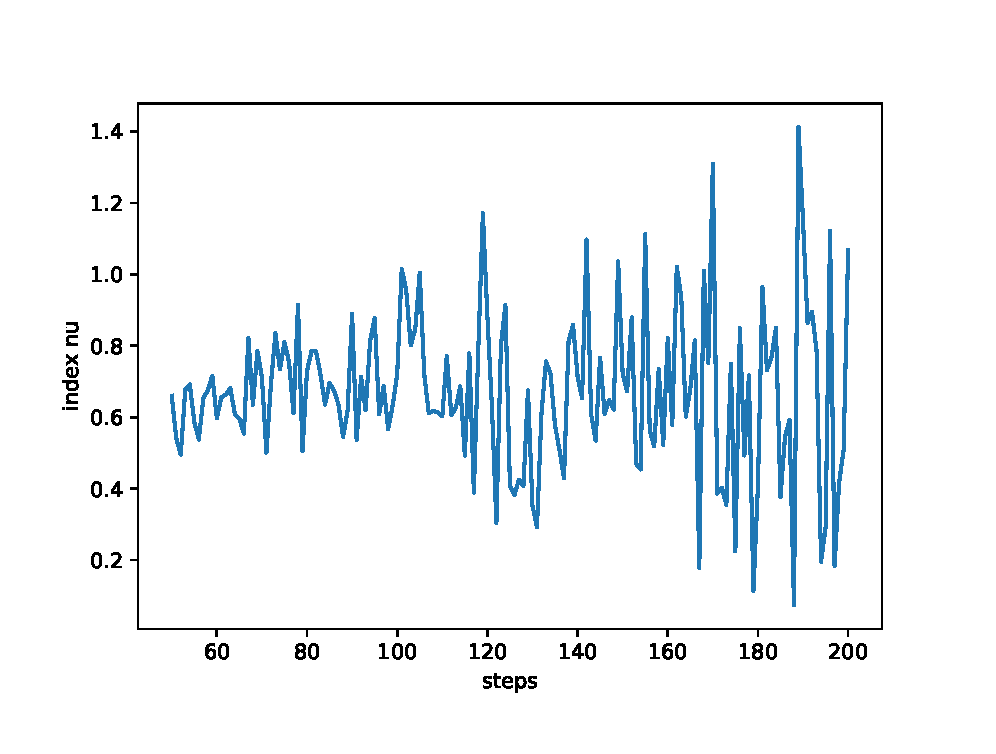
\includegraphics[width=0.8\textwidth]{fig1.eps}
    \caption{$N-\nu$关系图}
\end{figure}

计算结果有一定统计涨落,其中心值在0.7左右,这与一般(非自规避)RW的值($\nu=0.5$)相比
要更大,也就是说随着$N$增长,GSAW比普通RW相比$ \langle r^2(N) \rangle
$的值变大的更快,这与理论和直觉相符合.

\subsection{求指数$\gamma$值}

将计算出的$\gamma$指数展示如下:
\begin{figure}[!h]
    \centering
    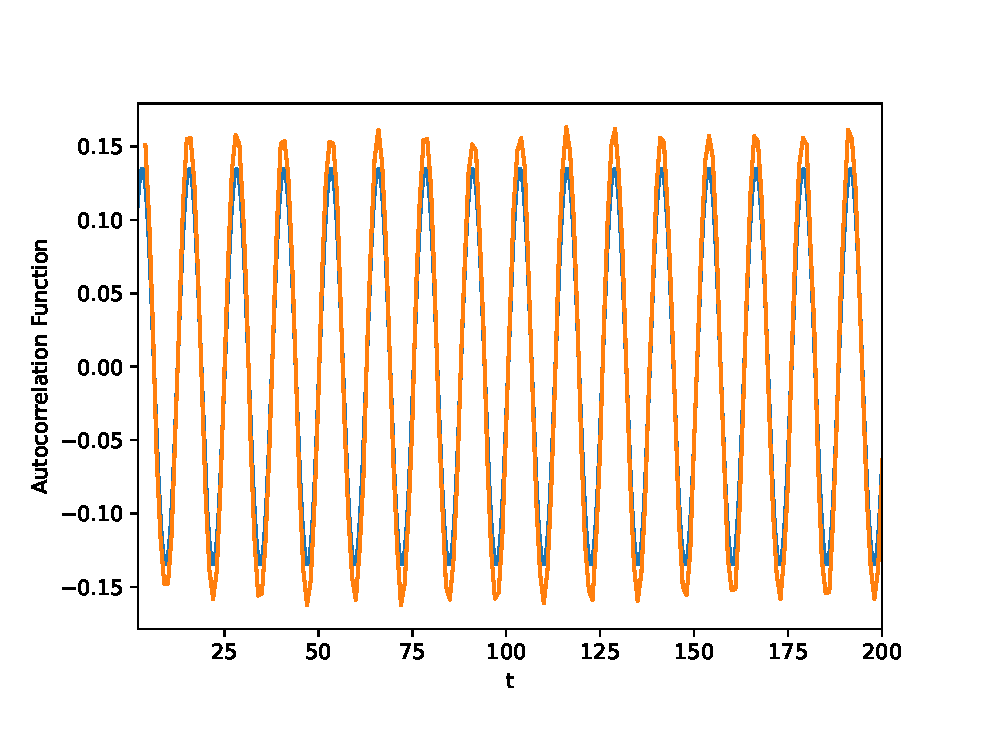
\includegraphics[width=0.8\textwidth]{fig2.eps}
    \caption{$N-\gamma$关系图}
\end{figure}

结果显示,指数$\gamma$值有较大的起伏,在0附近波动且随着$N$增大波动幅度越来越大.
这在一定程度上表明行走步数越大,一定步数所对应的行走数目与步数的关系越不确定,
增加或减少步数对随机行走数的影响越大,这可以理解为是SAW的约束性所导致的. 

\section{结论}

本题中我们一定程度上实现了GSAW的功能,并计算了相关指数与一般RW比较,
得出了GSAW的一些相关性质. 

\section{源代码}

FORTRAN90程序显示如下:
\begin{framed}
\begin{lstlisting}[language=Fortran]
MODULE RW
IMPLICIT NONE

CONTAINS
FUNCTION sqdr(steps) ! RW生成器函数,返回行走距离的平方sqdr
    INTEGER(KIND=4), INTENT(IN) :: steps
    INTEGER(KIND=4) :: i, j
    INTEGER(KIND=4) :: dir, lastdir, tmpr(2)
    INTEGER(KIND=4), DIMENSION(0:steps, 2) :: r
    INTEGER(KIND=4), DIMENSION(-steps:steps, -steps:steps) :: lattice
    REAL(KIND=8) :: sqdr
    LOGICAL(KIND=4) :: revive, reach
    REAL(KIND=8) :: seed, rand(steps), tmprand(50)

    reach = .FALSE.
    DO WHILE(reach .EQV. .FALSE.)
        CALL RANDOM_NUMBER(seed) !用FORTRAN自带的随机数生成器生成16807生成器的种子
        CALL Schrage(steps, int(2147483647 * seed), rand)
        r(0, :) = [0, 0]
        lattice = 0
        lattice(0, 0) = 1
        DO i = 1, steps
            IF(i .EQ. 1) THEN ! 第一步有4个可能方向
                dir = int(4 * rand(i)) ! 设dir=0,1,2,3分别对应向左,下,右,上
                r(i, :) = r(i-1, :) + walk(dir)
                lattice(r(i, 1), r(i, 2)) = 1 ! 将走过点对应的lattice值标记为1
                lastdir = dir
            ELSE ! 后面的步最多只能有3个可能方向
                dir = noturn(lastdir, int(3 * rand(i)))
                ! 从除了上一步行走方向反方向的3个选择中随机选择一个
                tmpr(:) = r(i-1, :) + walk(dir) ! tmpr表示粒子下一步可能前往的位置
                IF(lattice(tmpr(1), tmpr(2)) .EQ. 1) THEN
                    revive = .FALSE.
                    CALL RANDOM_NUMBER(seed) 
                    CALL Schrage(20, int(2147483647 * seed), tmprand)
                    ! 若抽中的方向将导致粒子死亡,再次抽样尽量避免这次死亡
                    DO j = 1, 50
                        dir = noturn(lastdir, int(3 * tmprand(j)))
                        tmpr(:) = r(i - 1, :) + walk(dir)
                        IF(lattice(tmpr(1), tmpr(2)) .NE. 1) THEN
                            r(i, :) = tmpr(:)
                            revive = .TRUE.
                            EXIT
                        END IF
                    END DO
                    IF(revive .EQV. .FALSE.) THEN
                        EXIT ! 如果粒子复活失败,则死亡
                    END IF
                ELSE
                    r(i, :) = tmpr(:)
                    lattice(r(i, 1), r(i, 2)) = 1
                END IF
                lastdir = dir
            END IF
            IF(i .EQ. steps) THEN
                reach = .TRUE.
            END IF
        END DO
    END DO
    sqdr = DOT_PRODUCT(r(steps, :), r(steps, :)) ! 求走过了指定步数RW距离的平方
END FUNCTION sqdr

FUNCTION Z(total, steps) ! 同为RW生成器函数,返回达到某指定步数粒子的比率
    INTEGER(KIND=4), INTENT(IN) :: total, steps
    INTEGER(KIND=4) :: successes, l, i, j
    INTEGER(KIND=4) :: dir, lastdir, tmpr(2)
    INTEGER(KIND=4), DIMENSION(0:steps, 2) :: r
    INTEGER(KIND=4), DIMENSION(-steps:steps, -steps:steps) :: lattice
    LOGICAL(KIND=4) :: revive
    REAL(KIND=8) :: seed, rand(steps), tmprand(50), Z

    successes = 0
    DO l = 1, total
        CALL RANDOM_NUMBER(seed) !用FORTRAN自带的随机数生成器生成16807生成器的种子
        CALL Schrage(steps, int(2147483647 * seed), rand)
        r(0, :) = [0, 0]
        lattice = 0
        lattice(0, 0) = 1
        DO i = 1, steps
            IF(i .EQ. 1) THEN ! 第一步有4个可能方向
                dir = int(4 * rand(i)) ! 设dir=0,1,2,3分别对应向左,下,右,上
                r(i, :) = r(i-1, :) + walk(dir)
                lattice(r(i, 1), r(i, 2)) = 1 ! 将走过点对应的lattice值标记为1
                lastdir = dir
            ELSE ! 后面的步最多只能有3个可能方向
                dir = noturn(lastdir, int(3 * rand(i)))
                ! 从除了上一步行走方向反方向的3个选择中随机选择一个
                tmpr(:) = r(i-1, :) + walk(dir) ! tmpr表示粒子下一步可能前往的位置
                IF(lattice(tmpr(1), tmpr(2)) .EQ. 1) THEN
                    revive = .FALSE.
                    CALL RANDOM_NUMBER(seed) 
                    CALL Schrage(20, int(2147483647 * seed), tmprand)
                    ! 若抽中的方向将导致粒子死亡,再次抽样尽量避免这次死亡
                    DO j = 1, 50
                        dir = noturn(lastdir, int(3 * tmprand(j)))
                        tmpr(:) = r(i - 1, :) + walk(dir)
                        IF(lattice(tmpr(1), tmpr(2)) .NE. 1) THEN
                            r(i, :) = tmpr(:)
                            revive = .TRUE.
                            EXIT
                        END IF
                    END DO
                    IF(revive .EQV. .FALSE.) THEN
                        EXIT ! 如果粒子复活失败,则死亡,进入下次循环
                    END IF
                ELSE
                    r(i, :) = tmpr(:)
                    lattice(r(i, 1), r(i, 2)) = 1
                END IF
                lastdir = dir
            END IF
            IF(i .EQ. steps) THEN
                successes = successes + 1 ! 成功走到最后则累计成功数successes
            END IF
        END DO
    END DO
    Z = real(successes) / total ! 计算成功比率
END FUNCTION Z

SUBROUTINE Getnu() ! 计算nu的子程序
    INTEGER(KIND=4) :: j, N, minim = 50, maxim = 200
    REAL(KIND=8) ,DIMENSION(50:200) :: nu
    REAL(KIND=8) :: big_ave = 0, small_ave = 0
    DO N = minim, maxim 
        print *, 'computing nu, ',N, 'steps / 200steps'
        DO j = 1, 300
            small_ave = small_ave - small_ave / j + sqdr(N-10) / j 
            big_ave = big_ave - big_ave / j + sqdr(N+10) / j 
            ! 分别累计r(N-i),r(N+i)的平均值,且防止溢出
        END DO
        nu(N) = 0.5 * LOG(big_ave / small_ave) / LOG(real(N+10) / real(N-10))
        ! 按照公式由双对数曲线斜率求指数nu(N)
    END DO
    OPEN (1, file='nu.dat') !将nu(N)数值写入文件
    WRITE (1, *) nu
    CLOSE (1)
    print *, 'Done with nu!'
    print *, '------------------------------------'
END SUBROUTINE Getnu

SUBROUTINE Getgam() ! 计算指数gamma的子程序
    REAL(KIND=8), DIMENSION(50:200) :: gam
    INTEGER(KIND=4) :: N, minim = 50, maxim = 200

    DO N = minim, maxim
        print *, 'computing gamma, ', N, 'steps / 200steps'
        gam(N) = 1 + (real(N) / 10)**2 * LOG(Z(10000, N)**2 / &
                (Z(10000, N-10) * Z(10000, N+10)))
    END DO
    OPEN (1, file='gamma.dat')
    WRITE (1, *) gam
    CLOSE (1)
    print *, 'done with gamma!'
END SUBROUTINE Getgam

FUNCTION noturn(lastd, r) !不走回上一步的方向选择器
    INTEGER(KIND=4) :: r, lastd
    INTEGER(KIND=4) :: noturn
    SELECTCASE(r)
        CASE(0)
            noturn = MOD(MOD(lastd + 2, 4) + 1, 4)
        CASE(1)
            noturn = MOD(MOD(lastd + 2, 4) + 2, 4)
        CASE(2)
            noturn = MOD(MOD(lastd + 2, 4) + 3, 4)
    END SELECT
    ! 一个两个相反方向对应数字的关系为: A=MOD(B+2, 4)
END FUNCTION noturn
FUNCTION walk(direction) ! 将数字代号转换成位移坐标的函数
    INTEGER(KIND=4) :: direction
    INTEGER(KIND=4), DIMENSION(2) :: walk
    SELECTCASE(direction)
        CASE(0)
          walk = [-1, 0]
        CASE(1)
          walk = [0, -1]
        CASE(2)
          walk = [1, 0]
        CASE(3)
          walk = [0, 1]
    END SELECT
END FUNCTION walk

END MODULE RW

SUBROUTINE Schrage(num, z0, rand) 
    !Schrage随机数生成器子程序,将均匀随机数序列存放在数组rand中
    IMPLICIT NONE
    INTEGER(KIND=4) :: N = 1, num
    INTEGER :: m = 2147483647, a = 16807, q = 127773, r = 2836, In(num), z0
    REAL(KIND=8), INTENT(INOUT) :: rand(num)
    In(1) = z0 !将传入值z0作为种子
    rand(1) = REAL(In(1))/m
    DO N = 1, num - 1
        In(N + 1) = a * MOD(In(N), q) - r * INT(In(N) / q)
        IF (In(N + 1) < 0) THEN !若值小于零,按Schrage方法加m
            In(N + 1) = In(N + 1) + m
        END IF
        rand(N + 1) = REAL(In(N + 1))/m !得到第N+1个随机数
    END DO

END SUBROUTINE Schrage

PROGRAM MAIN
    USE RW
    IMPLICIT NONE
    CALL Getnu() ! 调用求指数nu的子程序
    CALL Getgam() ! 调用求指数gamma的子程序
END PROGRAM MAIN
\end{lstlisting}
\end{framed}
\end{document}

